% !TEX root = ../main.tex

\chapter{A Shortfall in Investor Expectations of Leveraged Tokens}\label{ch:shortfall}

\textit{This chapter is based on the work ``A Shortfall in Investor Expectations of Leveraged Tokens'' ~\cite{shortfall} supervised by Dr. \supv and published in the sixth international conference on Advances in Financial Technologies (AFT 2024), at the Austrian National Bank (OeNB) in Vienna, Austria.}

\section{Introduction}
In this chapter, we present a summary of our research on Leveraged Tokens (LVTs) and discuss shortcomings such as deviation from leverage, higher fee and the risk of front-running. LVTs are emerging crypto-assets primarily issued by centralized exchanges. The concept is borrowed from leveraged ETFs (LETFs) in traditional financial markets, which offer higher gains (and higher losses) relative to price movements in the underlying asset. However, LVTs have been implemented differently from LETFs by exchanges in the crypto market, with variations across platforms.

We examine the mechanics and constituent components of LVTs, demonstrating that the lack of a standard has resulted in deficiencies and unexpected technical and economic outcomes. To identify existing problems, we analyze over 1,600 leveraged tokens from 10 issuers. Our analysis reveals that 99.9\% of LVTs are centralized, with 80\% lacking blockchain interaction, leading to transparency issues. Total supply information is difficult to access for 53\% of them, and 41\% appear inadequately backed at launch. Additionally, 97\% of LVTs are vulnerable to front-running during well-known events, and they deviate from their stated leverage ratios more than LETFs, partly due to inconsistent re-leveraging processes and higher management fees. This work provides a framework for crypto investors, blockchain developers, and data analysts to gain a deep understanding of leveraged tokens and their impact on market dynamics, liquidity, and price movements. It also offers insights for crypto exchanges and auditors into the internal functionalities and financial performance of LVTs under varying market conditions.

\section{Related Work}
The study of leveraged financial instruments has been extensively explored in traditional markets, particularly with Leveraged ETFs (LETFs). Prior research has shown that LETFs suffer from compounding effects, which distort their intended leverage over time, particularly in volatile markets~\cite{trainor2010,guedj2010,mackintosh2008,cheng2010,charupat2011}. Frequent rebalancing has been proposed as a necessary mechanism to maintain tracking accuracy, although it may introduce additional market inefficiencies~\cite{cheng2009,hill2009,leung2012}.

Moreover, the impact of LETFs on market liquidity and volatility has been widely studied, with findings indicating that daily rebalancing can create price distortions and increased trading volumes near market close~\cite{rompotis2016,shum2016,trainor2010,guedj2010,werner2022,kout2019}. Despite the extensive analysis of LETFs, there has been limited academic work on Leveraged Tokens (LVTs) in the cryptocurrency market. Some research has highlighted how investors often misunderstand the risks associated with leveraged instruments, emphasizing the need for better regulatory guidance and investor education~\cite{leung2012}.

Our study builds upon these prior works by conducting an extensive analysis of over 1,600 LVTs, identifying key deficiencies in transparency, leverage consistency, and financial backing. By bridging the gap between traditional leveraged instruments and their crypto counterparts, our work contributes to the understanding of LVTs’ structural issues and offers insights into their financial and regulatory implications.

\section{Motivation for Studying LVTs}
Since 2019, more than 1,600 LVTs have been issued by various crypto exchanges. The FTX exchange introduced the original concept by issuing 102 tokens on the blockchain. Trading volumes exceeded \$1 million per day~\cite{TradingVolume}. This upward trend has continued, with other exchanges issuing approximately 32 new LVTs per month on average from January 2020 to November 2023 (see Table \ref{tab:lvts}). Considering the growing trend of these tokens, it is important to study them from the following perspectives:
\ExecuteMetaData[sections/tables]{tab-lvts}

\begin{itemize}
	\item \textsl{LVT attractiveness for investors:} Investment in LETFs nearly doubled in 2022 compared to 2021~\cite{FT_LETF}, demonstrating an appetite for low-risk leverage, which is satisfied in the crypto market by LVTs. LVTs reduce liquidation risks compared to derivatives and margin trading. However, other characteristics (\eg volatility drag) must be understood to avoid unexpected value destruction. These risks are not unique to LVTs; they also exist in LETFs.\anote{risk}
	
	\item \textsl{LVT distinctive dynamics:} Understanding key aspects of LVTs, such as their underlying dynamics, peculiarities in product design, effects on crypto markets, and investor suitability. Leveraged products can impact market dynamics, especially in highly volatile markets~\cite{shum2016intraday}. Technical details on LVT mechanics can be also useful for those involved in the design and implementation of LVTs to understand how these tokens affect liquidity and price movements, potentially influencing the robustness and reliability of trading algorithms.
	
	\item \textsl{Regulatory implications:} LVTs introduce new risks for market regulation, investor protection, and financial stability. Our work contributes to broader discussions on how to effectively regulate emerging financial technologies like LVTs. Additionally, since LVTs are often held by commercial firms requiring audited financial statements~\cite{devault2021blessing}, auditors should understand how LVTs function, their risks, and how they perform under different market conditions.
\end{itemize}

It is worth mentioning that a single crypto-asset can be used to create multiple leveraged tokens, with each token representing a different leverage ratio or strategy. In our review of over 1,600 tokens, manual verification was not employed for every token; instead, data was aggregated through APIs, issuer websites, and platforms like cryptodatadownload.com. As a result, the analysis was conducted in clusters, grouping tokens based on common characteristics and leveraging automated tools to handle the large dataset efficiently.

\section{Leveraged Token Mechanics}\label{sec:mechanics}
LVTs are tokenized representations of a leveraged fund whose value is derived from the value of a leveraged product. Leveraged products are essential components of LVTs, allowing issuers to form a leveraged fund and offer it as centralized or decentralized tokens. 99.9\% of LVT issuers use crypto futures as the leveraged product. LVTs are intentionally designed with leverage as a core component of their architecture. They are aimed at outperforming the return of the underlying benchmark on a daily basis.\anote{performance} Let $P_{t_{n}}$ represent the LVT price at calendar time $t_{n}$, expressed as:
\begin{equation}\label{eq:price}
	P_{t_{n}}=P_{t_{n-1}}\left(1+k\frac{\Delta S_{t_{n}}}{S_{t_{n-1}}}\right) \quad n\in[1,365), t\ge0, k\in\left[-5,-0.5\right] \cup \left[0.5,5\right]
\end{equation}
$S_{t_{n}}$ is the underlying price at time $t_{n}$, indexed by $n$, where $n$ denotes the days of the year. The frequency of $n$ does not have to be daily; it can be redefined in hours or minutes without any loss of generality. However, since daily returns are embedded in the LVT product design, $n$ is effectively daily. $P_{t_{n}}$ represents the price of the LVT at the close of trading day $n$. $S_{t_{n-1}}$ and $P_{t_{n-1}}$ are the initial prices of the underlying asset and LVT, respectively, at the beginning of trading day $n$ (or at the end of trading day $n-1$). $\Delta S_{t_{n}}$ is the amount of change in the underlying price relative to the initial price. The constant variable $k$ is the LVT multiplier (leverage), which can be defined as either a fixed or dynamic value, depending on the issuer. LVTs with fixed leverage can take values from the set $\left\{-5,-3,-2,-1,-0.5,0.5,2,3,5\right\}$, while dynamic leverage fluctuates within the range $\left[-4.0, -1.25 \right] \cup \left[ 1.25, 4.0 \right]$.

To properly reflect the value of the fund through circulating LVTs, the notional value of all tokens must match the fund's notional value. As the price of the leveraged product changes over the trading day, the leverage of the fund gradually diverges from the stated ratio. The \textsl{fund management algorithm} resets this deviation by buying or selling the leveraged product on a daily basis. It also implements the logic of the LVT and defines how it should function in different market conditions. If an LVT is designed to be fully on-chain, the smart contract provides the functionality of this functionality, by extending common features of the ERC-20 standard. The constituent components of LVTs vary depending on the issuer. According to issuer documentation, the general components of a typical LVT are illustrated in Figure \ref{fig:components}, followed by a brief explanation of the functionality of each component.

\begin{figure}[t]
	\centering
	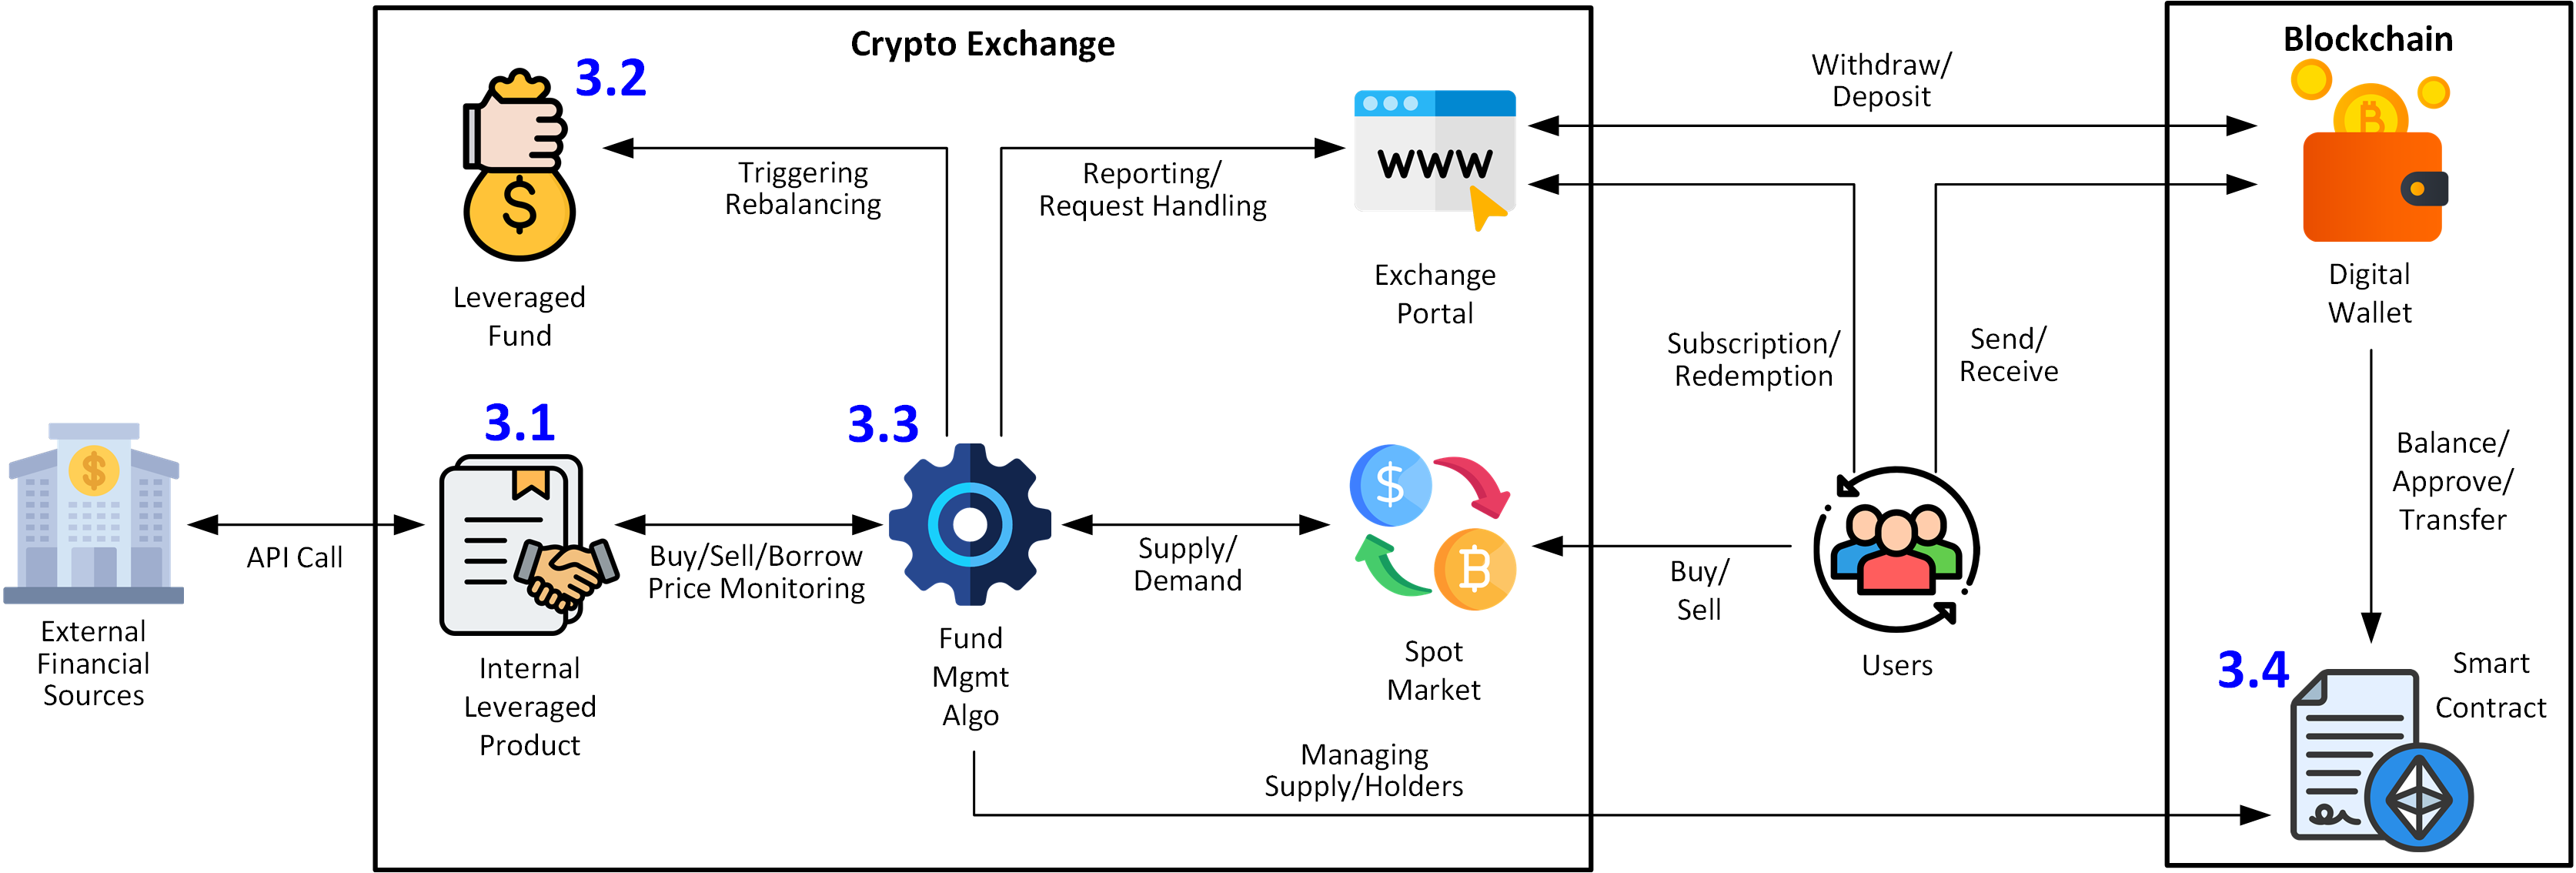
\includegraphics[width=0.98\textwidth,keepaspectratio]{components.png}
	\caption[LVT constituent components]{The constituent components of LVTs, according to the issuer's documentation. Some issuers have implemented them internally, resulting in missing blockchain components.}
	\label{fig:components}
\end{figure}

\subsection{Leveraged Product}\label{subsec:leveragedproduct}
Financial managers of LETFs use leverage to open positions worth more than the required capital. In LVTs, leveraged exposure can be achieved by (i) opening positions in the crypto derivatives market, which provides up to 200x leverage, and (ii) borrowing capital from external sources, generating up to 10x leverage. LVT issuers typically do not use high multiples, offering tokens with up to 5x leverage. This allows them to choose either derivatives or debt as the leveraged product. 99.9\% of issued LVTs use futures (a type of derivative), and only \textsl{Index Coop} uses the debt market to finance investments.\anote{coop-debt} The desired outcome for \textsl{Index Coop}'s tokens is to generate future returns that outweigh the cost of borrowing. Other issuers that use derivatives aim to minimize dependency on other exchanges for buying and selling futures. They often offer the corresponding futures trading in their own portfolio to facilitate LVT management and reduce the cost of transactions between exchanges (compare the \textsl{Leveraged Product} and \textsl{Fund Source} columns in Table \ref{tab:lvts}). For example, every issuer that launched BTC Long/Short tokens offers BTC-Perp futures as the underlying. Internal leveraged products facilitate LVT operations, such as adjusting fund positions, monitoring underlying price fluctuations, and triggering fund rebalancing.

\subsection{Leveraged Fund}\label{subsec:leveragedfund}
It is a fund that derives its \textsl{notional value} from a basket of leveraged products.\anote{notional} The leveraged products provide leveraged exposure, upon which the value of the issued tokens is based. Let $V_{t_{n}}$ represent the price of the $k$-times leveraged product $V$ on trading day $n$, tracking the underlying asset $S$. The price of $V_{t_{n}}$ differs from $S$ as it carries $k$-times exposure. A leveraged fund $L$ with a notional value of $L_{t_{n}}$ can be formed by purchasing a basket of $V$, given by:
\begin{equation}\label{eq:leveragedfund1}
	L_{t_{n}}=kV_{t_{n}}B_{t_{n}}\big(1+(\rho_{t_{n}}+\phi_{t_{n}})\big)\quad t \ge 0, \rho_{t_{0}}=0, \phi_{t_{0}}=0
\end{equation}
Where $B_{t_{n}}$ is the number of $V$ units forming the fund at the rebalancing time $t_{n}$. $\rho_{t_{n}}$ and $\phi_{t_{n}}$ represent management and futures funding fees, respectively. $\rho_{t_{n}}$ is always negative, as the issuer deducts associated expenses from the fund's value. $\phi_{t_{n}}$ can be positive or negative, depending on the \textsl{futures funding fee} payments (more in Section \ref{fundingfee}). The sum of $\rho_{t_{n}}$ and $\phi_{t_{n}}$ (\ie the total daily fee) varies per LVT issuer and ranges from 0.01 to 0.5 percent daily. Note that the change in the price of the leveraged product ($V_{t_{n}}$) is proportional to the underlying price ($S_{t_{n}}$), but does not vary based on the $k$ multiplier. More precisely, $V_{t_{n}} = V_{t_{n-1}}(1+R_{t_{(n-1)\to n}})$. In equation (\ref{eq:leveragedfund1}), $L_{t_{n}}$ represents the financial value controlled by the leveraged fund $L$, which originates from the leveraged product $V$. The change in the price of $V$ is proportional to $S$, but the value of $L$ changes with respect to the $k$ factor. In simple terms, $V$ represents the price of the leveraged product, while $L$ represents the amount of money that can be controlled using $V$.
\begin{example}\label{ex:eth2l_1}
	An issuer may arrange an \textsl{Ether long double-leveraged fund} by purchasing 4 \textsl{Ether-Perp long 2x futures} at \$1.5K ($V_{t_{0}}$). The 2x leverage of Ether-Perp allows the issuer to pay half of the Ether price, which is assumed to be \$3K ($S_{t_{0}}$). With zero fees in (\ref{eq:leveragedfund1}) at $t_{0}$ ($\rho_{t_{0}}+\phi_{t_{0}}=0$), a leveraged fund $L$ worth $2\times{\$1.5K}\times{4}=\$12K$ can initially be formed ($L_{t_{0}}$). A 10\% change in the price of Ether affects the price of futures by the same 10\%, bringing it to \$1.65K ($V_{t_{n}}$). However, the notional value of the fund ($L_{t_{n}}$) changes according to $k=2$, reaching $2\times{\$1.65K}\times{4}=\$13.2K$. This demonstrates the effect of $k$ on $L$ compared to $V$.
\end{example}

LVTs are issued with a certain initial supply that can be adjusted through the \textsl{Subscription} and \textsl{Redemption} process. For added or removed tokens, the issuer offsets the notional value of the fund with the notional value of the tokens by buying or selling the corresponding amount of the leveraged product. Let $N_{t_{n}}$ represent the total supply of a $k$-leveraged LVT at time $t_{n}$. The notional value of the issued LVTs ($A_{t_{n}}$) can be expressed as:
\begin{equation}\label{eq:leveragedfund2}
	A_{t_{n}}=kN_{t_{n}}P_{t_{n}}
\end{equation}
Equating (\ref{eq:leveragedfund1}) and (\ref{eq:leveragedfund2}) gives the total number of tokens ($N_{t_{n}}$) that should exist at the price of $P_{t_{n}}$ at time $t_{n}$. Mathematically, this can be expressed as: $kN_{t_{n}}P_{t_{n}}=kV_{t_{n}}B_{t_{n}} \Rightarrow  N_{t_{n}}=\frac{V_{t_{n}}B_{t_{n}}}{P_{t_{n}}},\quad t \ge 0, P_{t_{0}} \ge 1$.

\begin{example}\label{ex:eth2l_2}
	Assume $P_{t_{0}}=\$10$ as the initial offering price of ETH2L in the previous example \ref{ex:eth2l_1}. $P_{t_{0}}$ is typically set by the issuer at either \$1 or \$10 per token.\anote{IPO} The initial supply of ETH2L at \$10 per token is \(N_{t_{0}}=\frac{V_{t_{n}}B_{t_{n}}}{P_{t_{n}}}=\frac{\$1.5K\times{4}}{\$10}=600\). The notional value of all 600 tokens ($A_{t_{0}}=2\times{600}\times{\$10}=\$12K$) is consistent with the notional value of the leveraged fund ($L_{t_{0}}=2\times{\$1.5K}\times{4}=\$12K$). Investors purchase a portion of this fund in the form of LVT, allowing them to generate twice the profit compared to the underlying Ether-Perp. Essentially, the value of the ETH2L token is derived from the \textsl{Ether long 2x leveraged fund}, which in turn is derived from the 4 positions in the \textsl{Ether-Perp long 2x futures}.
\end{example}

\subsection{Fund Management System}\label{subsec:fundmgmt}
As the price of the leveraged product ($V_{t_{n}}$) fluctuates over time, the notional value of the leveraged fund ($L_{t_{n}}$) changes, causing the leverage ratio of the LVT to deviate from the stated leverage. Let $\tilde{k_{t_{n}}}$ represent the realized leverage ratio that the notional value of the tokens ($A_{t_{n}}$) represents at time $t_{n}$, expressed as $\tilde{k_{t_{n}}}=\frac{L_{t_{n}}}{N_{t_{n}}P_{t_{n}}}$.

\begin{example}\label{ex:eth2l_3}
	Referring to the first trading day of ETH2L in examples \ref{ex:eth2l_1} and \ref{ex:eth2l_2}, in which the price of Ether ($S_{t_{0}}$) increases by 10\%, the notional value of the fund ($L_{t_{n}}$) changes to $2\times{\$1.65K}\times{4}=\$13.2K$. The 2x leverage of the LVT increases its price by 20\%, rising to \$12 ($P_{t_{n}}$) from the initial \$10 ($P_{t_{0}}$). Since the LVT supply remains constant at 600 tokens, the leverage ratio of the fund drops from $2$x to $1.8$x. ($\tilde{k_{t_{n}}}=\frac{L_{t_{n}}}{N_{t_{n}}P_{t_{n}}}=\frac{\$13.2K}{600\times{\$12}}=1.8\overline{3}$).
\end{example}
The analysis above suggests that with the change in the price of the underlying ($S_{t_{n}}$) and subsequently the price of the leveraged product ($V_{t_{n}}$), the notional value of the leveraged fund ($L_{t_{n}}$) changes, and the realized leverage ratio of LVTs ($\tilde{k_{t_{n}}}$) becomes higher or lower than the stated leverage $k$. Mathematically, if $\mathbb{E}[\tilde{k_{t_{n}}}]$ represents the expected change in $\tilde{k_{t_{n}}}$ in relation to the underlying price change ($S_{t_{n}}$), applying equations (\ref{eq:price}) gives us:
\begin{equation}
	\mathbb{E}[\tilde{k_{t_{n}}}]=\frac{kV_{t_{n}}B_{t_{n}}(1+R_{t_{(n-1)\to n}})}{kN_{t_{n}}P_{t_{n}}}=\frac{V_{t_{n}}B_{t_{n}}(1+R_{t_{(n-1)\to n}})}{N_{t_{n}}P_{t_{n-1}}(1+kR_{t_{(n-1)\to n}})}\label{eq:expected}
\end{equation}
As the number of tokens ($N_{t_{n}}$) remains constant while the price of the underlying changes at a rate of $(1+R_{t_{(n-1)\to n}})$, the denominator of (\ref{eq:expected}) changes $k$-times faster (or slower) than the numerator, resulting in positive or negative leverage skewness. This highlights the need to re-leverage the fund on a daily basis, a process managed by the \textsl{fund management}.\anote{fund-mgmt}

Fund management is an off-chain algorithm (or on-chain for decentralized tokens) that dynamically adjusts the fund to maintain the leverage at the expected ratio. When the token's leverage increases, it sells some of the fund's positions to reduce the leverage and return it to the expected level. The majority of algorithms are off-chain with no interaction with the blockchain. The only on-chain instance is implemented by \textsl{Index Coop}~\cite{IndexCoop_FLI_01}. In addition to correcting the leverage, the algorithm interacts with other components to adjust supply, update balances, monitor the price of the underlying, and deduct daily fees.

\subsection{On-chain Contracts}
For decentralized LVTs, a smart contract represents the leveraged fund on the blockchain. It is typically implemented as an ERC-20 token~\cite{Interface,ansari2020implementation,shirole2020cryptocurrency}, allowing users to exchange LVTs on the blockchain without issuer intervention. As indicated in the \textsl{Blockchain Representation} column of Table \ref{tab:lvts}, 80\% of issuers have not created LVTs on the blockchain. As a result, this component is missing from Figure \ref{fig:components}. The absence of a smart contract leads to several deficiencies, which are discussed in the next section.

\section{Deficiencies of Existing LVTs}
Due to the lack of a common standard in LVTs for defining the rebalancing process, data transparency and interoperability, these tokens are issued with varying features at the discretion of the issuer. We examine the characteristics of issued tokens per issuer and discuss the respective deficiencies as research questions RQ1 to RQ6.

\subsection*{RQ1: What information is visible to traders of an LVT?}\label{subsec:blockchain}
Among the 10 LVT issuers, only \textsl{FTX} and \textsl{Index Coop} have created tokens on the Ethereum blockchain. FTX's management model was hybrid (\ie tradable decentralized tokens on a centralized exchange), while only \textsl{Index Coop}'s tokens are fully decentralized. The remaining 8 exchanges prefer to implement LVTs centrally and entirely internal.
\begin{example}
	Binance leveraged tokens (BLVTs) are one of the centralized LVTs that are entirely accessible within Binance's ecosystem. They can be exclusively traded on Binance's spot market with no possibility of withdrawal. BLVTs are not even published on Binance's own blockchain (BNB Smart Chain) and are created more like a pseudo-crypto.\anote{Pseudo}
\end{example}

\subsubsection{Transparency in Total Supply}
Total supply is used to calculate the Net Asset Value (NAV) of LVTs as a representation of the market's fair value. Due to imbalances in supply and demand, the market price of LVTs may deviate from the NAV, trading at a premium or discount. In the long run, LVT prices converge to the NAV due to a mechanism similar to arbitrage in traditional markets. Orders placed far from the NAV price lose or gain value over time. In the short run, however, investors use the NAV as a reference price when buying or selling, especially in bulk. The NAV of LVTs can be calculated by equating (\ref{eq:leveragedfund1}) and (\ref{eq:leveragedfund2}), with the current token supply $N_{t_{n}}$:
\begin{equation}\label{eq:nav}
	kN_{t_{n}}P_{t_{n}}=kV_{t_{n}}B_{t_{n}} \Rightarrow  P_{t_{n}}=\frac{V_{t_{n}}B_{t_{n}}}{N_{t_{n}}}\quad t \ge 0, N_{t_{0}} \ge 1
\end{equation}
\begin{example}
	In the previous examples (\ref{ex:eth2l_1}) to (\ref{ex:eth2l_3}), when the Ether price increases by 10\% on day 2, the market price of ETH2L trades at \$12 (after a $2\times{10\%}=20\%$ increase), while its NAV price is $(\$1.65K\times{4})/600=\$11$. ETH2L is, in fact, overvalued, and traders should wait for either (i) the arbitrage mechanism to play out and bring the LVT price down, or (ii) the next rebalancing schedule, which will match the fund's value with the notional value of the tokens.
\end{example}

For LVTs hosted on the blockchain, total supply is public and can be retrieved for NAV calculations. However, for centralized LVTs, investors must refer to the exchange's website. The total supply of tokens on some exchanges, such as AscendEX, Pionex, Gate.io, and ByDFi, does not appear to be public, making it difficult to verify the real value of LVTs (\ie 53\% of all tokens). LVTs are \textsl{open-end funds} with a theoretically unlimited token supply.\anote{open-end} Issuers can increase the supply based on market liquidity and demand for the token. Transparency in the number of issued tokens builds trust and reduces the risk of investment. Moreover, it addresses audit questions such as, Has the fund's value changed proportionately after increasing or decreasing the supply of LVTs? How much were the fund's value deviations in the previous audit period, and were they within the acceptable range?

\subsubsection{Transparency in Transactions}
Transactions on the blockchain show the flow of tokens and the movement of the fund. This enables investors to analyze transactions and ensure the expected functionality of LVTs.

\begin{example}
	We reviewed all \textsl{Mint} and \textsl{Burn} transactions of ETCBULL (FTX 3x Long Ethereum Classic) on the blockchain.\anote{FTX-ETCBULL} The analysis suggests that a total of 51,640,895 tokens were issued, and 24,207 were destroyed (\ie 51,616,688 circulating tokens). The trend of issuing tokens has taken on exponential velocity since April 2022. A total of 783,022 tokens were issued during the 960-day period between October 2019 and May 2022, while 50,857,873 tokens were issued over just 184 days from April to October 2022. In other words, 98.5\% of all tokens were issued in just 6 months. Checking the recipient address indicates FTX's possible sub-wallet as the receiver. This sudden change in token supply warrants further investigation, especially given FTX's collapse shortly afterward.
\end{example}

This is just an example indicating the importance of transparency in LVT transactions. Transactions of centralized tokens are not public and only available to the issuer. Statistically, transactions of 80\% of LVTs cannot be analyzed as we did in the above case.

\subsubsection{Transparency in Token Holders}
Holders of tokens created on the blockchain are public, allowing investors to check them as a measure of the token's liquidity. A small number of market participants reduces the token's liquidity and can make it more challenging to execute large orders. It may also lead to a wider bid-ask spread, increasing the cost of executing trades. Investors generally prefer assets with higher liquidity, narrower bid-ask spreads, and more market participants.
\begin{example}
	90\% of XRPBULL (FTX 3x Long Ripple) tokens are distributed among four holders.\anote{FTX-XRPBULL} In another example, three accounts own 94\% of all issued FTX 3x Long Cardano (ADABULL) tokens.\anote{FTX-ADABULL}
\end{example}

Holding a large number of tokens by a limited number of accounts can noticeably elevate investment risk. One holder may decide to sell a significant number of tokens at any moment, potentially resulting in a notable price drop within a short period of time, leading to significant losses for smaller holders. Since most issuers do not publish the list and respective ownership percentages of centralized LVTs, the participants of 80\% of LVTs remain uncertain.

\subsubsection{Inability to Audit}\label{sec:audit}
Conducting audits ensures the security, functionality, and compliance of LVTs as claimed by the issuer. Unlike centralized LVTs, the code of tokens created on the blockchain is public, allowing auditors to identify vulnerabilities and associated risks. The security of these 20\% decentralized LVTs can be evaluated by reviewing the code against industry best practices such as SWC~\cite{SWC}. Moreover, external audits are essential for LVTs to ensure they function as intended, such as verifying the output of methods when transferring tokens or updating balances. Auditors may also provide recommendations to improve the security, functionality, and compliance of LVTs. For centralized LVTs, the code is not public, requiring cooperation and willingness of the issuer to conduct a thorough review and quality assessment. Sharing the code and the results of an independent audit would improve transparency and help build trust between token holders and issuers.

\subsection*{RQ2: To what extent are LVTs locked to the exchange?}\label{subsec:exchange}

\subsubsection{Interoperability with dApps and DeFi}
In 2019, the total value locked in Decentralized Finance (DeFi) was approximately 700 million USD. As of April 2022, it stands at around 150 billion USD, representing more than 200\% growth in less than three years~\cite{werner2022sok}. Hosted LVTs on the blockchain (which usually comply with one of the fungible\anote{fungible} token standards) facilitate interaction with DeFi systems, unlocking potential interoperability opportunities. 
\begin{example}
	FTX was able to employ blockchain interoperability to share its ETHBULL (3x Long Ether) with other exchanges such as Poloniex, Indodax, Bittrex, and Gate.io.\anote{FTX-ETHBULL} These exchanges owned 20\%, 4\%, 3\%, and 2\% of ETHBULL, respectively, and offered it on their platforms due to the possibility of interaction with DeFi.
\end{example}
In contrast, centrally issued LVTs cannot interact with other platforms and operate in isolation, preventing LVTs from moving across different platforms. Decentralized LVTs, on the other hand, foster connectivity and enable users to access a wide range of services and functionalities without being confined to a single exchange.

\subsubsection{Inability to Custody}
At first glance, the custody issue seems common to all assets on centralized exchanges. However, BTC buyers can transfer it to their personal wallets, while centralized LVTs remain locked within the exchange. Holders do not own the actual tokens but are simply betting on price movements. Some explain this custodial issue by viewing LVTs as ``token contracts'', though this term is not widely recognized nor aligns with the functionality of crypto derivatives. LVTs are essentially tokenized forms of derivative exposures.
\begin{example}
	BTCUP and BTCDOWN are issued by Binance and track Bitcoin as the underlying asset. Unlike Bitcoin holders, owners of these tokens cannot withdraw or transfer them to their own digital wallets. In contrast, similar Bitcoin leveraged tokens were created by FTX on the Ethereum blockchain (known as BULL and BEAR tokens). Holders of these tokens still had the opportunity to exchange them on decentralized exchanges, such as Uniswap\anote{FTX-DEX}, shortly after FTX's bankruptcy. Holders could recover 80\% of the token value on the first day of the bankruptcy, 50\% on the second day, and up to 20\% on the third day.
\end{example}

\subsection*{RQ3: Are the LVTs offered today adequately backed?}\label{subsec:backing}
The simplest definition of an LVT is a tokenized leveraged fund. According to the documentation of LVT issuers, 99.9\% of leveraged funds derive their value from a basket of positions in the futures market~\cite{AscendEX_Guide,MEXC_Guide,Binance_Guide,ByBit_Guide,ByDFi_Guide,FTX_Guide,GateIO_Guide,KuCoin_Guide,Pionex_Guide}. The issuer must either (i) offer futures trading in their portfolio, or (ii) open futures positions on other crypto exchanges and manage them systematically through APIs as the underlying asset fluctuates.\anote{pionex-binance} The question we raise, due to the lack of external audits, is to what extent LVT issuers have properly prepared futures contracts before launching LVTs. Have users invested in tokens that are properly backed, or are they simply trusting the issuer and potentially investing in tokens with no real value?

\subsubsection{Missing Futures Product}
Some issuers have launched LVTs without offering the corresponding futures products. While we cannot rule out the possibility that they hold the necessary futures positions on other exchanges, this raises concerns that these LVTs might not be adequately backed financially.

\begin{example}
	AscendEX uses its own futures products and does not rely on futures products from other exchanges. However, they issued 3x/5x Long/Short Monero (XMR3L/S and XMR5L/S) without offering XMR perpetual contracts initially. To our knowledge, no XMR futures products were available on the market from any exchange to be used as leveraged products at the time of the launch of these XMR tokens.
\end{example}

The above example is one of 390 issued tokens lacking a corresponding futures product (see column B of Table \ref{tab:missing}). Based on available historical data and information from the issuer's website, 24\% of LVTs did not have the necessary futures product offered by the same issuer and instead relied on futures from other exchanges.

\ExecuteMetaData[sections/tables]{tab-missing}

\subsubsection{Delayed Futures Product}
Missing futures products are not the only issue with centralized LVTs. For 264 tokens, the corresponding futures product was only offered after the issuance of the tokens (see column A of Table \ref{tab:missing}). In other words, at the time of the launch of 17\% of LVTs, the required futures may not have existed. According to the LVT documentation on issuers' websites, these issuers did not disclose using futures from other crypto exchanges. Internal futures trading was introduced later, after the token was launched.

\begin{example}
	MEXC issued 3x Long/Short Cardano (ADA3L/S) in February 2020, while ADA-Perp was only launched in July 2020, resulting in a 154-day delay. They did not disclose using futures from other exchanges, indicating the fund might have been operating without financial backing during this period.
\end{example}

According to available information, on average, 41\% of LVTs have missing or delayed futures products (see column E of Table \ref{tab:missing}). The main financial issue with LVTs is the lack of transparency in the fund management system. Centralized LVTs function like a black box to investors and are fully managed by the issuer. Even for tokens with proper futures backing (\eg Binance, ByBit, and KuCoin), investors can rely solely on numeric assertions made on the issuer's website.

\subsection*{RQ4: What are the possibilities of front-running?}\label{subsec:frontrunning}
Front-running is an illegal practice in the equity market where non-public information is used to purchase shares of a company before the price moves~\cite{eskandari2019sok,zhou2021high,baum2022sok}. For instance, FINRA\anote{FINRA} announced a \$700K fine against \textsl{Citadel Securities}\anote{CITADEL} in 2020 for front-running activities between 2012 and 2014~\cite{Investo_FrontRunning}. In the design of LVTs, certain well-known events can be exploited by traders to benefit from anticipated price movements. They can engage in similar front-running practices that may impact the price of the underlying asset and the token itself. We review these events and explore possible front-running scenarios as follows.

\subsubsection{Event I: Impending Fund Rebalancing}\label{subsec:rebalancing}
To keep the leverage at the stated ratio, issuers perform periodic rebalancing. This can be triggered at predefined intervals (\eg every day, every 8 hours, or every $n$ blocks), or upon meeting certain conditions (\eg after exceeding a specific threshold). All LVT issuers perform regular daily rebalancing and trigger interim rebalancing in volatile markets (see columns B and C of Table \ref{tab:missing}). They may trigger rebalancing when the underlying asset's price fluctuates by more than $X\%$, or when the leverage passes a threshold. The \textsl{fund management algorithm} governs the rebalancing process, adjusting futures positions and restoring the leverage ratio to the target level.

The number of contracts that must be bought or sold to restore the leverage is predictable, making front-running possible. Let $\Delta B_{t_{n}}$ represent the number of required futures contracts to rebalance the fund at time $t_{n}$. $\Delta B_{t_{n}}$ can be easily calculated by considering the return of the underlying asset from time $t_{n-1}$ to $t_{n}$ ($R_{t_{(n-1)\to n}}$). The number of required futures contracts to restore the fund leverage can be calculated by subtracting the notional value of the tokens (equation \ref{eq:leveragedfund2}) from the notional value of the fund (equation \ref{eq:leveragedfund1}):
\begin{equation*}
	\resizebox{.95\hsize}{!}{$
		\Delta{B_{t_{n}}}=(1+kR_{t_{(n-1)\to n}})kN_{t_{n-1}}P_{t_{n-1}}-(1+R_{t_{(n-1)\to n}})kV_{t_{n-1}}B_{t_{n-1}}-(\rho_{t_{n}}+\phi_{t_{n}})L_{t_{n}}+\epsilon_{t_{n}}
		$}
\end{equation*}
This equation is quadratic and can be simplified as $ax^2 - bx - c$ for long tokens, and $-ax^2 + bx - c$ for short tokens. When the underlying return is positive ($R_{t_{(n-1)\to n}} > 0$), $\Delta{B_{t_{n}}}$ is always positive ($a > 0$), and when the return of the underlying is negative, $\Delta{B_{t_{n}}}$ is negative as well ($a < 0$). In simpler terms, for long LVTs, futures exposure must be increased when the underlying price is rising, and decreased when the underlying price is falling.

There is also a fund expenses term $(\rho_{t_{n}} + \phi_{t_{n}})L_{t_{n}}$, which is usually deducted from the fund's value to cover operating expenses. However, this term can turn positive when the received funding fees ($\phi_{t_{n}}$) exceed the fund expenses ($\rho_{t_{n}}$). $\epsilon_{t_{n}}$ represents a disturbance term that captures the effects of news or shocks in the underlying. Since rebalancing is a predictable event, by buying or selling $\Delta{B_{t_{n}}}$ of the leveraged product, other traders can front-run the trade, potentially impacting the price of the token or even the underlying asset.

\begin{example}
	Consider the following sequence in which Alice calculates $\Delta{B_{t_{n}}}$ to potentially front-run the rebalancing trade:
	
	\begin{enumerate}
		\item Alice checks the issuer's website for the upcoming rebalancing of BTC5L (5x Long Bitcoin). She notices the next daily rebalancing is scheduled for 00:00 UTC.
		\item Alice calculates the number of contracts that will be bought or sold by the issuer to maintain the 5x target leverage of BTC5L.
		\item Alice front-runs the rebalancing trade by placing an order just before 00:00 UTC (ahead of the rebalancing trade). If she anticipates that the algorithm will buy Bitcoin futures, she may buy Bitcoin futures expecting increased demand, driving up the price, and giving her the opportunity to sell futures at higher prices. Conversely, if BTC5L will be selling the fund's positions, leading to increased supply, she may sell Bitcoin futures.
	\end{enumerate}
	Front-running in the above example may not only manipulate the price of Bitcoin futures but also inflate the price of BTC5L. Consider the following scenarios (A) and (B), with corresponding calculations in Table \ref{tab:frontrunning}.
	
	\begin{itemize}
		\item Alice calculates the \textsl{Basket Delta} of BTC5L prior to the rebalancing schedule and realizes that the algorithm will purchase 594.21 new contracts at \$33,000 (Scenario A in Table \ref{tab:frontrunning}). Assuming this purchase increases the price of Bitcoin futures by 1\%, she can buy contracts just before the rebalancing trade at \$33,000 and sell them afterward at \$33,330. A 1\% increase in the underlying price inflates the token price to \$15.05. This provides Alice an additional opportunity to buy the token for \$15 before the rebalancing and sell it at a higher price afterward.
		
		\item The effect of Alice's strategy in the previous scenario may be amplified if many traders engage in front-running. The increased demand may raise the price of Bitcoin futures even before the rebalancing trade. If the influx of other traders pushes Bitcoin futures up by 1\%, and the rebalancing trade further increases the price by another 1\%, this secondary effect could also inflate the token price further and create more price distortion (Scenario B in Table \ref{tab:frontrunning}).
	\end{itemize}
\end{example}

\ExecuteMetaData[sections/tables]{tab-frontrunning}

\subsubsection{Event II: Management Fee Deduction}
Similar to LETFs, daily fees and expenses are deducted from the leveraged fund to cover associated costs. The fee rate and daily schedule vary by issuer (see columns D and E of Table \ref{tab:missing}). Management fees are deducted at specific times, allowing adversaries to exploit this known event, potentially coinciding with rebalancing. The simultaneous occurrence of events I and II can intensify the front-running effect during the rebalancing process.

\begin{example}
	Consider the same sequence as the previous example, where Alice calculates the \textsl{Basket Delta} of BTC5L at the same time as the management fee deduction. The issuer's withdrawal of \$99,000 (Management fee row in Table \ref{tab:frontrunning}) reduces the fund's value. To compensate, \$99,000/\$33,000 = 3 additional contracts need to be purchased. The coincidence of these two events causes the rebalancing algorithm to slightly increase demand by purchasing 597.21 contracts instead of 594.21.
\end{example}

\subsubsection{Event III: Futures Funding Fee Exchanges}\label{fundingfee}
Funding fee is a mechanism in Perps to converge the price of contracts with the price of the underlying crypto. It is calculated based on the notional value of the futures position and is exchanged between short and long traders who keep their positions open. Shorts pay longs when the funding rate is negative, and longs pay shorts when the rate is positive(see \ref{appx:funding} for more details). The intervals for \textsl{Funding fee exchange} are public and displayed on the issuer's website, typically occurring every 8 hours at 00:00 UTC, 08:00 UTC, and 16:00 UTC. Since the fund is composed of futures, it either pays or receives funding fees at these times. This predictably increases or decreases the value of the leveraged fund, which can be exploited to amplify the effects of front-running.

The impact of front-running can be exacerbated when events I, II, and III occur simultaneously. Such concurrency may force the algorithm to buy or sell more contracts than would be required for fund rebalancing alone (\ie $\Delta{\tilde{B_{t_n}}}=\sum_{n=1}^{3}{\Delta{B_{t_{n}}}}$).

\begin{example}
	As calculated in the \textsl{Basket Delta} row of Table \ref{tab:frontrunning}, in the first rebalancing cycle, an additional 2.70 futures contracts are required to cover the 0.3\% daily management fee deduction and 0.03\% daily funding fee exchange. This means that 2.7 more contracts will be added if events II and III coincide with event I. The impact on basket delta can be even more significant as the value of the fund increases in a volatile market.
\end{example}

To mitigate front-running in LVTs, issuers should avoid rebalancing the fund on predetermined schedules. Techniques such as intraday or randomized rebalancing, or algorithmic trading, can help reduce the visibility of rebalancing trades.\anote{iceberg} Only Binance avoids regular daily rebalancing, instead triggering it when the underlying price fluctuates more than 10\% or when leverage falls outside the range of $\left[-4.0, -1.25 \right] \cup \left[ 1.25, 4.0 \right]$. This means 97\% of current LVTs perform fund rebalancing at specific intervals, increasing the likelihood of daily front-running (see column B of Table \ref{tab:missing}).

\subsection*{RQ5: How well do LVTs track their asserted leverages?}\label{subsec:deviation}
The leverage ratio of LVTs is determined by the issuer and can be either variable (dynamic) or fixed. If an LVT uses the \textsl{Underlying+Leverage+Long/Short} naming convention, the leverage is most likely fixed. The \textsl{Underlying+Up/Down} format is used for LVTs with variable leverage.
\begin{example}
	KuCoin has issued ETH3L as a 3x long token tracking Ether as the underlying. Binance similarly offers ETHUP and ETHDOWN tokens with a target leverage in the range of [1.25, 4] and [-4, -1.25], respectively.
\end{example}

Very high leverage factors such as $\pm10$x or $\pm15$x are not common in currently issued LVTs, as the majority of them provide $\pm3$x leverage. Low leverage is aimed at minimizing losses and extending the liquidation point during periods of high volatility. Highly leveraged LVTs lose value in the same proportion as the underlying asset and may not be attractive to investors. Crypto exchanges advertise LVTs as an investment vehicle providing leveraged exposure to crypto-assets with minimal liquidation risk. However, LVTs with high leverage factors defeat this promise.

\subsubsection{Inconsistency of Fixed Leverage}
Approximately 16\% of LVTs are issued with variable leverage, fluctuating in the range of $\left[-4.0, -1.25 \right] \cup \left[ 1.25, 4.0 \right]$. Additionally, 9\%, 59\%, and 11\% of LVTs have fixed 2x, 3x, and 5x leverage ratios, respectively. As shown in Table \ref{tab:deviation}, LVTs with fixed leverage may not always provide exactly the promoted leverage. One aspect of risk involves leverage deviation (also called tracking error). Furthermore, some issuers do not rebalance the fund in the same way.

\ExecuteMetaData[sections/tables]{tab-deviation}

\begin{example}
	MEXC and KuCoin adjust the leverage of only the tokens that have lost value. Consider a volatile market where Bitcoin loses 10\% in a day. These issuers adjust only the leverage of BTC3S, while the leverage of BTC3L remains unchanged, as it gained value~\cite{MEXC_Guide,KuCoin_Leverage}. For example, if the price of Bitcoin is \$30K and the fund holds 600 contracts, the fund's initial value is \$18M. Assuming 600K issued tokens at an initial offering price of \$10, the target leverage is 3x (\ie \(k=(600\times{\$30K})/(600K\times{\$10})=3\)). A 10\% increase in Bitcoin's price changes the leverage of BTC3L and BTC3S to 2.53x and 4.71x, respectively. However, these exchanges correct the leverage of BTC3S to prevent further capital loss in case of more price decline. As a result, this rebalancing process undervalues the BTC3L fund (\ie inflates the value of BTC3L). Instead of only rebalancing the losing side, both BTC3L and BTC3S positions should be adjusted simultaneously to bring the leverage back to 3x as advertised by the issuer.
\end{example}

We compared the leverage deviation of Bitcoin LVTs with LETFs over the course of a year. Analysis details are provided and Table \ref{tab:deviation}. As can be seen, LVTs exhibit higher leverage deviations than similar products in the equity market. This issue becomes more apparent when comparing the standard deviation of returns in the equity and crypto markets. 

Leverage deviation leads to underperformance or overperformance of tokens, causing investors to experience returns that deviate from the intended amplification effect of LVTs. This is particularly important in light of previous research on LETF returns, which shows that LETFs, on average, do not negatively impact investor short-term returns~\cite{loviscek2014leveraged}. Results indicate that the daily return distribution using real-world historical data is significantly more leptokurtic than the normal distribution. However, in LVTs, returns tend to have a wider or flatter shape (platykurtic) due to higher leverage deviation.

\subsubsection{Disadvantages of Variable Leverage}
LVTs with variable leverage aim to: (i) minimize the impact of volatility drag, and (ii) reduce the possibility of front-running (as discussed in Section \ref{subsec:frontrunning}). LVTs are advertised as an investment vehicle that amplifies returns relative to a certain multiplier, although this factor changes constantly in tokens with variable leverage. This introduces an additional risk dimension, requiring regular monitoring and adjustment of positions as the leverage fluctuates. 

Additionally, these types of tokens rebalance on an as-needed basis with no predetermined schedules. Rebalancing can be triggered by (i) a sudden fluctuation in the underlying price (such as more than 15\%), (ii) exceeding the expected leverage range (such as above 4x or below 1.25x for long LVTs), and (iii) handling subscription or redemption requests, which change the total supply. One disadvantage of this type of rebalancing is that funds can remain undervalued or overvalued for extended periods.

\ExecuteMetaData[sections/tables]{tab-gap}

\begin{example}
	The rebalancing events of BTCUP (a Long BTC LVT by Binance) over the past 3 years are listed in Table \ref{tab:gap}. A rebalancing event occurred on 03-Jan-2023, 204 days after the previous one on 13-Jun-2022. During those 204 days, no rebalancing event was triggered because the changes in Bitcoin’s price did not exceed the 10\% threshold limit, and the fund’s leverage fluctuated within the expected range of [1.25x, 4x]. During this period, the fund’s value was much lower (or higher) than the amount required to support the value of issued tokens, but no rebalancing occurred. Undervalued funds may benefit the issuer, while investors hold inflated tokens.
\end{example}

Another disadvantage of dynamic leverage is the imbalance in rebalancing triggers. Some issuers initiate the rebalancing at different ranges for long and short tokens.
\begin{example}
	Pionex triggers rebalancing when the leverage of long tokens exceeds the range of $\left[2.2, 4.0\right]$, while this range is $\left[1.8, 4.8\right]$ for short tokens~\cite{Pionex}. This inconsistency increases the complexity of position management, leading to unfavorable outcomes for investors.
\end{example}

Dynamic leverage may reduce the chances of front-running in LVTs but at the expense of token transparency and complicating position management. Each issuer puts in place its own algorithm for rebalancing of LVTs with dynamic leverage, since there is no uniform standard for the rebalancing process. This might be confusing for investors who switch from one issuer to another one, expecting similar performance.

\ExecuteMetaData[sections/tables]{tab-fee}

\subsection*{RQ6: Are LVT fees in-line with traditional LETFs?}\label{subsec:fees}
Issuers of LETFs/LVTs charge daily fees to compensate for the associated cost of operating the fund. Over the past few years, these fees have generally come down on average, where the Management Expense Ratio (MER) for traditional ETFs and LETFs annually averaged 0.45\% and 0.95\%, respectively. We investigated the daily fees for Bitcoin LVTs, and summarized our findings in Table \ref{tab:dailyfees}. 

The annual MER for these LVTs ranges from 1.83\% to 36.5\% depending on the issuer. By contrast, the standard deviation of MER in LETFs and LVTs is 0.38\% and 34.21\%, respectively. That would indicate that the fees for LVTs are less predictable and more volatile than for LETFs-by as much as 90-fold. This impacts the overall expense ratio and net returns of LVTs. Additionally, high fees typically characterize a market in its development stage with a limited issuer base. This may signal some risk for investors who would expect to see low fees once the market starts to mature and face some competition.

\section{Contributions}
In particular, the purpose of this chapter is not limited to introducing LVT but conducting an in-depth study from the underlying, interaction with blockchains, types of leveraged products, and algorithms for managing funds. We investigated more than 1,600 LVTs offered by 10 different issuers. Then, with a careful explanation of the mechanics and constituent components of LVT, readers would be able to understand how leveraged fund works, the rebalancing mechanism, and smart contracts in LVTs. Based on this, we answer the following six research questions about LVTs:

\paragraph{RQ 1: What information is visible to traders of an LVT?} In some of the centralized LVTs, important parameter such as the total supply, transactions, and holders not available to investors. Total supply an essential parameter for calculation of the tokens' fair value. It is also used by auditors when assessing the consistency and efficiency of LVTs. Transparency of the transactions helps investors, auditors, and all participants of the LVT ecosystem to analyze token flow, detect suspicious activity, enhance security, ensure compliance, and verify whether tokens are working the way they should be. Centrally issued tokens do not show how many holders there are, and their investment risks are much higher compared to their decentralized counterparts.

\paragraph{RQ 2: To what extent are LVTs locked to the offering exchange?} The inability to self-custody of centralized LVTs raises more concerns compared to their decentralized counterpart. It also increase the risk of investment in those crypto-assets. Another important advantage of tokens issued on the blockchain is their good interoperability with other dApps, crypto exchanges, and in general with the DeFi ecosystem. The LVTs interacting with DeFi enable tapping into new opportunities of participation in a more open and transparent financial system operating without intermediaries.
	
\paragraph{RQ 3: Are the LVTs offered today adequately backed?} The value of LVTs is derived from the value of a leveraged fund, which in itself is derived from the value set by futures. As no futures existed at such a point when the LVTs were offered, some investors may be investing in LVTs, which have either an inadequate or no financial backing. The analysis of publicly available historic data from the issuer's website gives evidence that on average, out of each 5 LVTs issued, 2 were seemingly not fully financially covered at the time of their issuance. Although over time, the exchange might have been addressed the issue, but at the time of issuance, required futures contracts were not offered by the exchange. Without external audits, investors must take the exchange's word for it and hope LVTs are indeed financially backed.
	
\paragraph{RQ 4: What are the possibilities of front-running in LVTs?} Predictability of front-running arises during fund rebalancing, deductions of management fees, and futures funding fee exchanges. An attacker would be able to take advantage of brief distortions in supply and demand created by the fund rebalancing trade. The effect could be amplified if all three events happen around the same time or multiple traders participate in the front-running practice at very high volumes. Front-running has also been an issue with LETFs, that is minimized due to constant monitoring by regulatory bodies like the SEC and FINRA.
	
\paragraph{RQ 5: How well do LVTs track their asserted leverage ratios?} While the value of the underlying changes, the value of the fund and the reflected leverage change at different rates. The token price may be at a premium or discount against the actual fund value. All the LVT issuers have a daily rebalancing schedule that reconciles the sum of the tokens' value and that of the fund. However, different issuers implement this process in a different way. This results in the actual effective leverage deviating from the target leverage. Rebalancing mechanism in both fixed and dynamic LVTs has some drawbacks. Fixed leverage is considered more suitable for LVTs as close to 100\% of all traditional LETFs use a fixed leverage factor~\cite{ETFDB}. However, applicable algorithms in LVTs should be revised to decrease the already high deviation of leverage from LETFs.
	
\paragraph{RQ 6: Are LVT fees in-line with traditional LETFs?} High daily fees in LVTs are a constant drag, eroding returns and causing underperformance. It also makes LVTs less attractive investment vehicles. Daily costs in LVTs should be much lower when compared to LETFs, since futures transactions occur internally and there is very little regulatory overhead. Besides that, higher fees are indicative of developing markets with low competition and inefficient cost management.

\section{Discussion}
Similar to leveraged ETFs, the foremost objective of LVTs is making leveraged investment easier while minimizing the hassle of managing such positions and limiting liquidation risks. In the course of our study, we found many shortcomings with LVTs-mostly not transparent, custodied with the issuing exchange, and may be inadequately backed. 99.9\% of LVTs are deployed as centralized products, available only within the ecosystem of the exchange itself. 80\% of them do not interact with the blockchain at all; due to this, there is no transparency in total supply, transactions, and holders. Some of these issues, along with various financial and security concerns in LVTs, were reviewed.

Since the issuers of 53\% of the LVTs do not publish their total supply, it is challenging for most investors to figure out the NAV and trade it at a fair price. Apart from this, 41\% of LVTs may also be launched without financial backing as the necessary futures contracts happen to be issued too late or may not have existed when the LVT was initially issued. 97\% of total LVTs are susceptible to front-running during generally known events. It enables the adversary to take advantage of rebalancing trades. Moreover, LVTs have higher leverage deviation from the stated ratio due to either inconsistency in management in token funds with fixed leverage or inefficiency in the rebalancing algorithm in LVTs with dynamic leverages. Generally speaking, LVTs have higher management fees compared to LETFs, which eats into the return of the fund in order for it to achieve the expected return. Due to the compounding effect, LVTs tend to underperform over an extended period of time, such as a month or a week, making them unsuitable as a long-term investment.

In fact, all our findings say the same: investors expecting simple leveraged positions that ``just work'' will be disappointed by leveraged tokens. Due to their peculiar properties, LVTs can only be safely used after considering them carefully, and as such, it is best for sophisticated traders.

Increased scrutiny by regulators and compulsory audits may be other ways to compel LVTs to be adequately backed. The fact that on-chain LVTs exist would allow self-custody and for greater transparency with respect to supply, transactions, and holders. For example, front-running mitigation should be explored using randomized rebalancing or using stealth trading (\eg iceberg orders). The LVT algorithms should also be modified to decrease deviations from the stated leverage. In summary, incorporating these methods better align LVTs with the natural investor expectations that they create. We implement all of these enhancements in a new hybrid design, LeverEdge, which we describe in detail in Chapter \ref{ch:leveredge}.